\documentclass[%
	12pt,%
	]
	{article}
\pagestyle{empty}
\usepackage[margin=1in]{geometry}
\usepackage{fancyhdr}
\usepackage{graphicx}
\usepackage{titlesec}
\usepackage{array}
\usepackage{textgreek}
\usepackage{newtxsf}
\usepackage{fontawesome}
% Uncomment next 2 lines to use TeX Gyre Heros sans serif
\usepackage{tgheros,tgtermes}
\renewcommand{\familydefault}{\sfdefault}
\titleformat{\section}
  {\normalfont\Large\bfseries}{\thesection}{1em}{}[{\titlerule[1.5pt]}]
  
\titleformat{\subsection}
  {\normalfont\Large\bfseries}{\thesubsection}{1em}{}[{\titlerule[0.5pt]}]

\usepackage{parskip,multicol}
\usepackage{xcolor}
\usepackage
	[%
        bookmarks=true,         % show bookmarks bar?
	unicode=false,          % non-Latin characters in Acrobat's bookmarks
	pdftoolbar=true,        % show Acrobat's toolbar?
	pdfmenubar=true,        % show Acrobat's menu?
	pdffitwindow=false,     % window fit to page when opened
	pdfstartview={FitH},    % fits the width of the page to the window
	pdftitle={Johanan Idicula's CV},    % title
	pdfauthor={Johanan Idicula},     % author
	pdfsubject={CV},   % subject of the document
	pdfcreator={Johanan Idicula},   % creator of the document
	pdfproducer={Johanan Idicula}, % producer of the document
	pdfkeywords={CV, Johanan, Idicula}, % list of keywords
	pdfnewwindow=true,      % links in new PDF window
	colorlinks=true,       % false: boxed links; true: colored links
	linkcolor=red,          % color of internal links (change box color with linkbordercolor)
	citecolor=red,        % color of links to bibliography
	filecolor=magenta,      % color of file links
	urlcolor=blue ,          % color of external links
	%
	]
	{hyperref}%

\title{\bfseries\Huge Johanan Idicula}
\author{\tt{\faEnvelopeO{} \href{mailto:johanan.idicula@mail.mcgill.ca}{johanan.idicula@mail.mcgill.ca}} \\ \tt{\faGlobe{} \href{https://jidicula.github.io/}{jidicula.github.io}}}
\date{} % delete this line to display the current date

\newcolumntype{L}{>{\raggedleft}p{0.14\textwidth}}
\newcolumntype{R}{p{0.8\textwidth}}

%%% BEGIN DOCUMENT
\begin{document}

\begin{minipage}{0.65\textwidth}
\begingroup
\maketitle
\endgroup
\end{minipage}                  % Don't put space between minipage environments!
\begin{minipage}{0.3\textwidth}
  \flushright{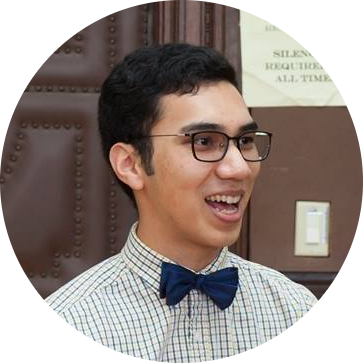
\includegraphics[width=0.8\textwidth]{../images/avatar_circle.png}} 
\end{minipage}

\pagestyle{fancy}
\setlength\headheight{14pt}
\fancyhead[r]{Updated \today}


\thispagestyle{fancy}

I'm a 4th year \href{http://www.mcgill.ca/anatomy}{Anatomy and Cell Biology} student at McGill University in Montr\'eal, Qu\'ebec. I'm also an undergraduate research assistant at the \href{http://bam.lab.mcgill.ca/}{Biological and Active Materials Lab} under the supervision of Professor Allen J. Ehrlicher in the McGill Department of Bioengineering.

\section*{Research Interests}

Cell Mechanics, \href{http://bam.lab.mcgill.ca/project_pages/ACTN4_Mechanosensitivity.html}{Mechanotransduction}, Gene Editing via CRISPR, ACTN4, Quantitative Imaging, Image Processing

\section*{Lab Skills}

\href{https://jidicula.github.io/images/micropattern.jpg}{Microcontact Printing}, Quantitative Confocal Microscopy, Mammalian Cell Culture, Plasmid Purification, Bacterial Cell Culture, Traction Force Microscopy, Image Processing


\section*{\href{https://github.com/jidicula}{Languages I Know}}

\textbf{Programming:} Python, MATLAB, Bash, Java, R

\textbf{Markup:} HTML, CSS, LaTeX

\textbf{Natural:} French (conversational and basic reading)

\section*{Tools I Use}

Git, TravisCI, Emacs, Eclipse, Atom, FIJI, scikit-image

\section*{Other Skills}

Strong writing and critical thinking

Careful attention to detail

Excellent proofreading and editing

Narration

\section*{Web Design}
\href{https://jidicula.github.io/macssmcgill/index.html}{MACSS}

\href{https://sarinalalla.github.io/}{Sarina Lalla's E-portfolio}

\section*{Education}
\begin{tabular}{LR}
{\bf 2014--2018}&{\bf B.Sc. Anatomy and Cell Biology, McGill University, Canada}\\[5pt]
2011--2014&International Baccalaureate Diploma, Colonel Gray High School, Canada.\\
\end{tabular}

\section*{Awards}
\subsubsection*{2018 McGill Anatomy and Cell Biology Research Retreat Undergraduate Travel Award}
Award covering cost of attendance at annual research retreat for trainees and faculty members in the McGill Department of Anatomy and Cell Biology.

\subsubsection*{2014 J.W. McConnell Entrance Scholarship}
McGill entrance scholarship for high school academic performance covering tuition and fees for the first year of the undergraduate degree.

\section*{Posters and Talks}

\begin{tabular}{LR}
  {\bf 2018-07-06}&{\bf Probing the Mechanosensitivity of \textalpha-actinin-4 Nuclear Translocation}\\[5pt]
                  &Poster presented at the 2018 ACB Annual Departmental Retreat, McGill University.\\[5pt]
  {\bf 2018-04-05}&{\bf Probing the Mechanosensitivity of \textalpha-actinin-4 Nuclear Translocation}\\[5pt]
                  &Talk presented at the McGill Integrative Bioscience Society Research Symposium, McGill University.\\[5pt]
  {\bf 2017-06-08}&{\bf Probing the Mechanosensitivity of ACTN4 nuclear translocation}\\[5pt]
                  &Talk presented at the 7th Annual Quantitative Life Science Symposium, McGill University.\\[5pt]
\end{tabular}

\end{document}
